Cette section présente l’architecture de notre solution, conçue pour garantir la cohérence, la performance, la maintenabilité et la scalabilité de l’application. Elle repose sur une architecture en trois tiers, typique des applications web modernes, intégrant des services conteneurisés et orchestrés afin d’optimiser le développement, le déploiement et l’exécution.

L’architecture s’articule autour de trois couches principales:
\begin{itemize}[label=$-$]
    \item \textbf{Couche de présentation (Frontend)}: développée avec \textbf{Angular} (version 18), cette couche constitue l’interface utilisateur accessible via un navigateur web, sur le port \textbf{4200}. L’application est conteneurisée à l’aide de \textbf{Docker} et servie par un serveur web \textbf{NGINX} sur le port \textbf{80}, garantissant rapidité et sécurité côté client. Elle suit le modèle \textbf{\acs{MVVM}} (Model-View-ViewModel)\cite{mvvm}:
            \begin{itemize}[label=$\circ$]
                    \item \textbf{Model}: définit les structures de données via des interfaces \texttt{TypeScript}, représentant les entités métier (utilisateurs, scans, résultats...).
                    \item \textbf{View}: composants visuels construits en \texttt{HTML}/\texttt{CSS}, correspondant à la partie graphique de l’application.
                    \item \textbf{ViewModel}: représenté par les \textbf{Components} Angular (liaison entre données et vue) et les \textbf{Services} (logique métier côté client, communication avec le backend).
            \end{itemize}
        En complément, le frontend s’appuie sur plusieurs mécanismes clés assurant la sécurité, la modularité et l’interactivité de l’application:
        \begin{itemize}[label=$\circ$]
            \item \textbf{Guards et routing Angular}: sécurisent la navigation à travers un système de routes hiérarchisées, protégées selon l’état d’authentification et le rôle de l’utilisateur.
            \item \textbf{Services Angular}: centralisent les interactions avec l’API REST (via \texttt{HttpClient}) et les traitements locaux (authentification, stockage, notifications, WebSocket).
            \item \textbf{Modèles TypeScript}: définissent les formats d’échange avec le backend, alignés avec les schémas \texttt{Pydantic} de FastAPI, pour faciliter la sérialisation/désérialisation des données.
            \item \textbf{WebSocket}: permet une communication bidirectionnelle en temps réel pour recevoir les mises à jour instantanées (progression des scans, alertes système).
        \end{itemize}
    \item \textbf{Couche applicative (Backend)}: développée avec \textbf{FastAPI}, elle est accessible via le port \textbf{8000} pour les requêtes \acs{HTTP}, et le port \textbf{8001} pour les communications \textbf{WebSocket}. Elle assure la logique métier, le traitement des requêtes, l’exposition des services web REST, l’interfaçage avec la base de données, la gestion de l’authentification et la coordination entre les autres couches.
    L’application est conteneurisée à l’aide de \textbf{Docker} et déployée via un \textbf{serveur Uvicorn} conforme à l’interface \textbf{\acs{ASGI}}, utilisé pour exécuter l’application \textbf{FastAPI}. Ce serveur gère efficacement les requêtes \acs{HTTP}/\acs{HTTPS} et les transmet aux routes définies dans FastAPI. Il prend également en charge les communications asynchrones via les \textbf{WebSockets}, ce qui le rend particulièrement adapté aux applications modernes nécessitant des échanges en temps réel.
    \begin{enumerate}[left=-0.03cm]
        \item \textbf{Les composants principaux de fastapi sont\cite{fastapiArc}}:
            \begin{itemize}[label=$\bullet$, left=-0.08cm]
                \item \textbf{Routes:} définissent les points d'entrée de l'\acs{API} REST, organisés par fonctionnalité et reçoivent les requêtes \acs{HTTP}.
                \item \textbf{CRUD}: Contiennent la logique métier et le traitement des données.
                \item \textbf{Models:} représentent les entités de la base de données sous forme de classes SQLAlchemy (\acs{ORM}).
                \item \textbf{Schemas Pydantic:} utilisés pour la validation et la sérialisation des données, ils définissent la structure des informations échangées (requêtes et réponses) entre le client et l’API.
                \item \textbf{\acs{DAO} (Data Access Objects)}: basé sur \textbf{SQLAlchemy} pour accéder à la base de données PostgreSQL, en assurant le mapping objet-relationnel (ORM).
                \item \textbf{JWT / OAuth2:} mécanisme d’authentification sécurisé reposant sur l’utilisation de \textbf{\acs{JWT}} (JSON Web Tokens) en combinaison avec le protocole \textbf{\acs{OAuth2}}, permettant la gestion des sessions, le contrôle des accès et l’attribution des rôles utilisateurs.
                \item \textbf{Canal WebSocket}: utilisé pour la communication en temps réel avec les utilisateurs, il permet à ces derniers de recevoir des mises à jour instantanées (notifications, état des scans, messages système...).
            \end{itemize}
        \item \textbf{Composants spécifiques ajoutés pour ce projet:}
            \begin{itemize}[label=$\bullet$, left=-0.08cm]
                \item \textbf{File de messages RabbitMQ + Workers}: fonctionne sur le port \textbf{5672} (port par défaut pour le protocole \acs{AMQP}) et expose une interface d’administration sur le port \textbf{15672}. Ce système permet le traitement asynchrone des tâches lourdes, telles que la gestion des scans, en répartissant la charge entre un pool de \textbf{workers asynchrones}. Les requêtes sont placées dans une file d’attente, puis traitées selon un nombre limité de tâches concurrentes afin de garantir les performances et la stabilité du système.\\
                Ce mécanisme permet de:
                \begin{itemize}[label=$\circ$]
                    \item Enregistrer les requêtes de scan dans RabbitMQ.
                    \item Traiter les tâches de façon asynchrone via un nombre fixe de \textbf{workers}.
                    \item Garantir une répartition équitable des ressources (N scans simultanés maximum).
                    \item Notifier l’utilisateur en temps réel une fois le traitement terminé.
                \end{itemize}
                Il favorise ainsi la scalabilité et prévient la saturation du système.
                \item \textbf{Service \acs{SMTP}}: utilisé pour l’envoi d’e-mails via le port \textbf{587} (TLS), selon la configuration du serveur SMTP.
                \item \textbf{Intégration \acs{Slack}}: notifications automatiques envoyées sur un canal Slack configuré via Webhook pour informer en temps réel des événements critiques (début/fin de scan, erreurs, vulnérabilités détectées).
                \item \textbf{Intégration Jira}: création automatique de tickets dans Jira lors de la détection de vulnérabilités critiques ou bloquantes, avec transmission des détails techniques (type, niveau de risque, description, solution proposée) depuis le backend.
               \item \textbf{Outils de sécurité}: L’application intègre plusieurs outils de scan automatisé, chacun exécuté dans un conteneur \textbf{Docker} isolé afin de garantir la modularité et l’évolutivité. Parmi ces outils, OWASP ZAP est accessible via le port \textbf{8080}, utilisé pour l’API et le proxy web. Les autres outils SQLMap, Wapiti, Nikto, Nuclei, Nmap, XSStrike, PwnXSS, WafW00f et WhatWeb sont lancés via des commandes dans leurs conteneurs Docker respectifs, sans ports exposés, car ils ne fonctionnent pas comme des services persistants. Les résultats sont ensuite centralisés, structurés et unifiés afin de pouvoir être exploités par d’autres modules tels que l’affichage, le reporting ou les alertes.
                \item \textbf{Outils pour les tests fonctionnels et audits SEO automatisés}:  
                    \begin{itemize}[label=$\circ$]
                        \item \textbf{Selenium}: utilisé pour simuler des interactions complexes avec des navigateurs web (navigation authentifiée, clics, remplissage de formulaires) afin de vérifier le comportement fonctionnel de l’application. Exécuté via un conteneur (\texttt{selenium/standalone-chrome}) sur le port \textbf{4444} (WebDriver).
                        \item \textbf{BeautifulSoup}: bibliothèque Python, utilisé pour analyser le DOM des pages web, permettant de détecter les balises et attributs essentiels à l’indexation (titres, meta description, balises \textit{alt}, structure \acs{HTML}...).
                    \end{itemize}                
            \end{itemize}
    \end{enumerate}
    \item \textbf{Couche de données}: assurée par une base de données relationnelle \textbf{PostgreSQL}, accessible via le port \textbf{5432}, elle stocke l’ensemble des informations de l’application, telles que les comptes utilisateurs, les résultats des scans, les historiques et les notifications. L’accès aux données est réalisé via des modèles \textbf{ORM (SQLAlchemy)}, garantissant la cohérence entre les entités logicielles et les tables relationnelles.
\end{itemize}
\noindent Tous les services (Angular, FastAPI, PostgreSQL, RabbitMQ, WebSocket...) sont conteneurisés avec \textbf{Docker} et orchestrés via \textbf{Docker Compose}, utilisant un réseau virtuel interne (bridge Docker) pour assurer une communication fluide entre les conteneurs.

La figure \ref{fig:architecture} illustre l’architecture de notre application en mettant en évidence les interactions entre ses différentes couches.
\begin{figure}[H]
    \centering
    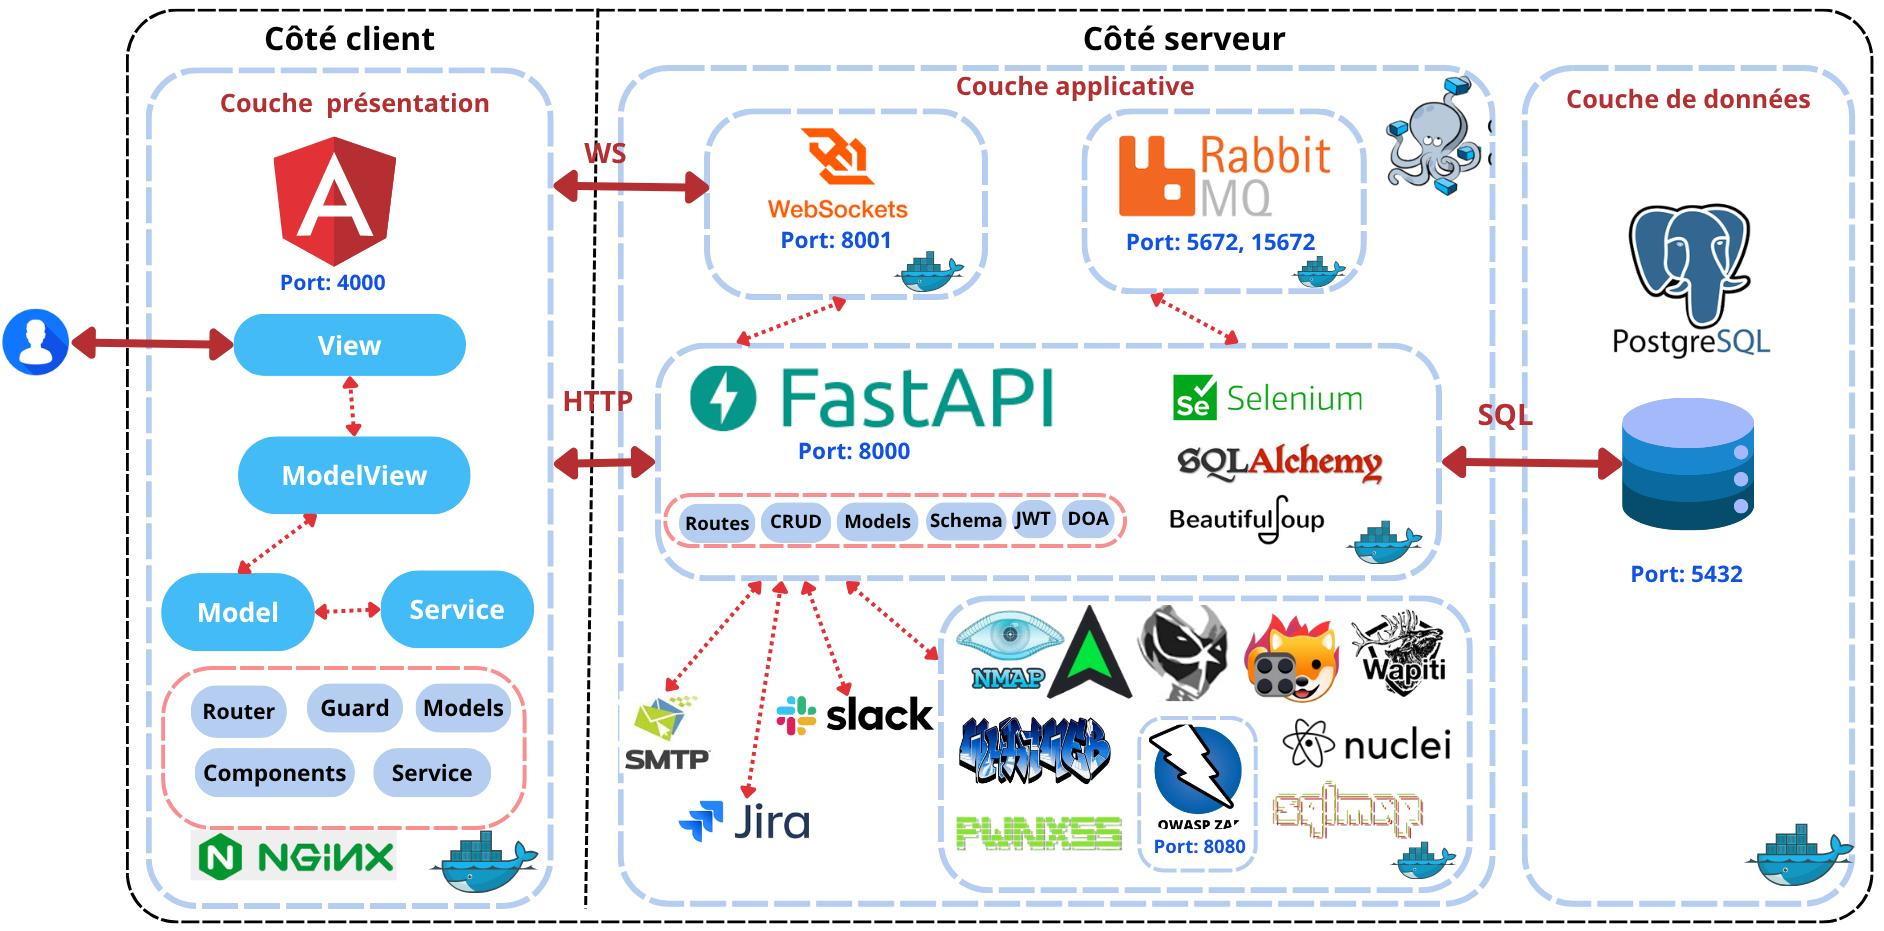
\includegraphics[width=\linewidth]{chapitres/ch2/img/architecture.png}
    \caption{Architecture de l’application}
    \label{fig:architecture}
\end{figure}
\vspace{-0.8cm}
\noindent Cette architecture conteneurisée garantit une haute disponibilité, la sécurité et la performance du système. Elle facilite la maintenance et l’évolution du projet, tout en assurant une scalabilité grâce à une séparation claire des responsabilités et à l’utilisation de services indépendants.